\documentclass{lug}

\title{Computer Graphics \& OpenGL}
\author{Sam Sartor}
\institute{Mines Linux Users Group}

\usepackage{etoolbox}
\usepackage{array}
\usepackage{amsmath}
\usepackage{adjustbox}

\makeatletter
\patchcmd{\beamer@sectionintoc}{\vskip1.5em}{\vskip0.5em}{}{}
\makeatother

\newcommand{\pmidg}[1]{\parbox{\widthof{#1}}{#1}}

\begin{document}

\section{Introduction}

\begin{frame}{Definition}
\begin{center}
    \pmidg{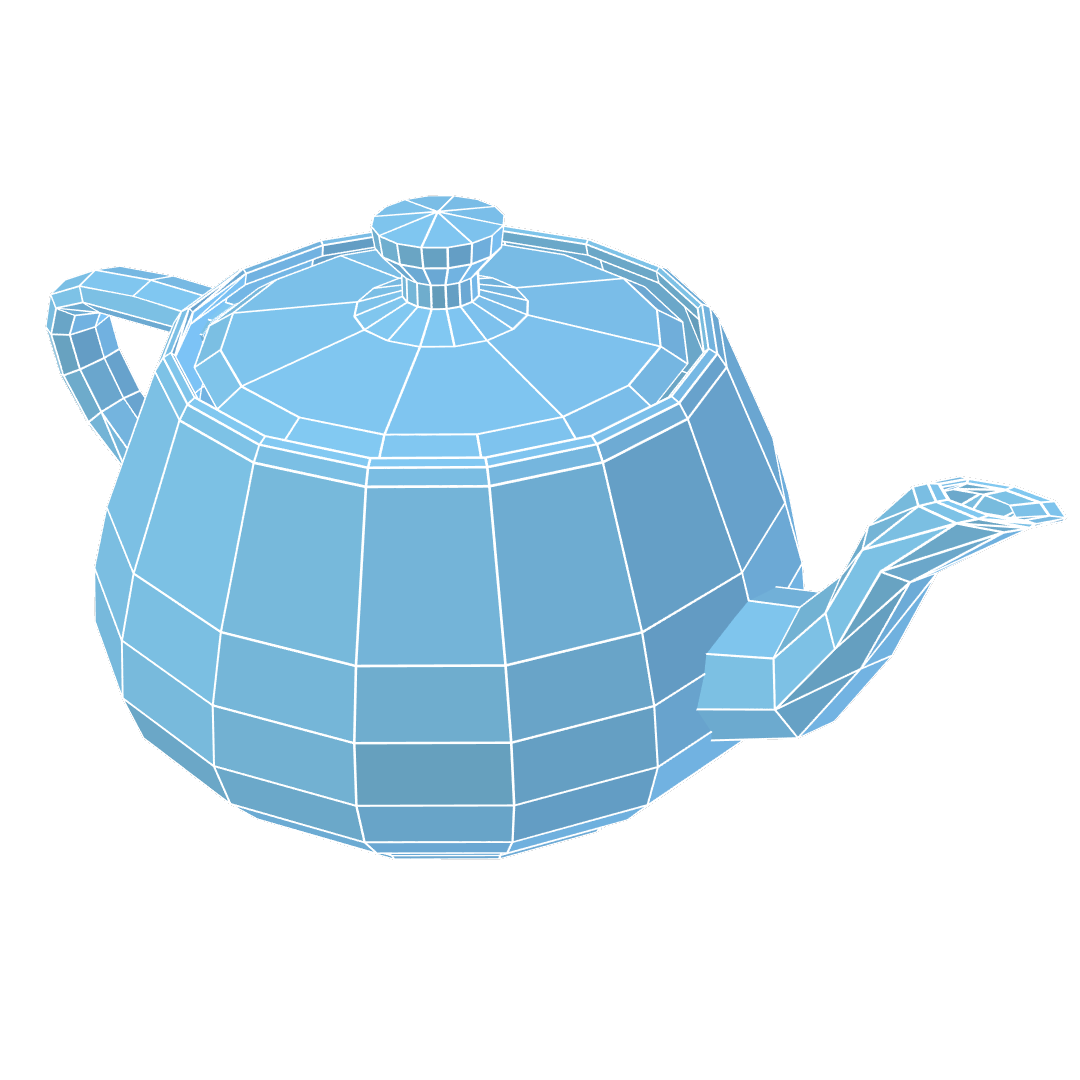
\includegraphics[width=4cm]{graphics/teapot_mesh}} \scalebox{2}{$\rightarrow$} \pmidg{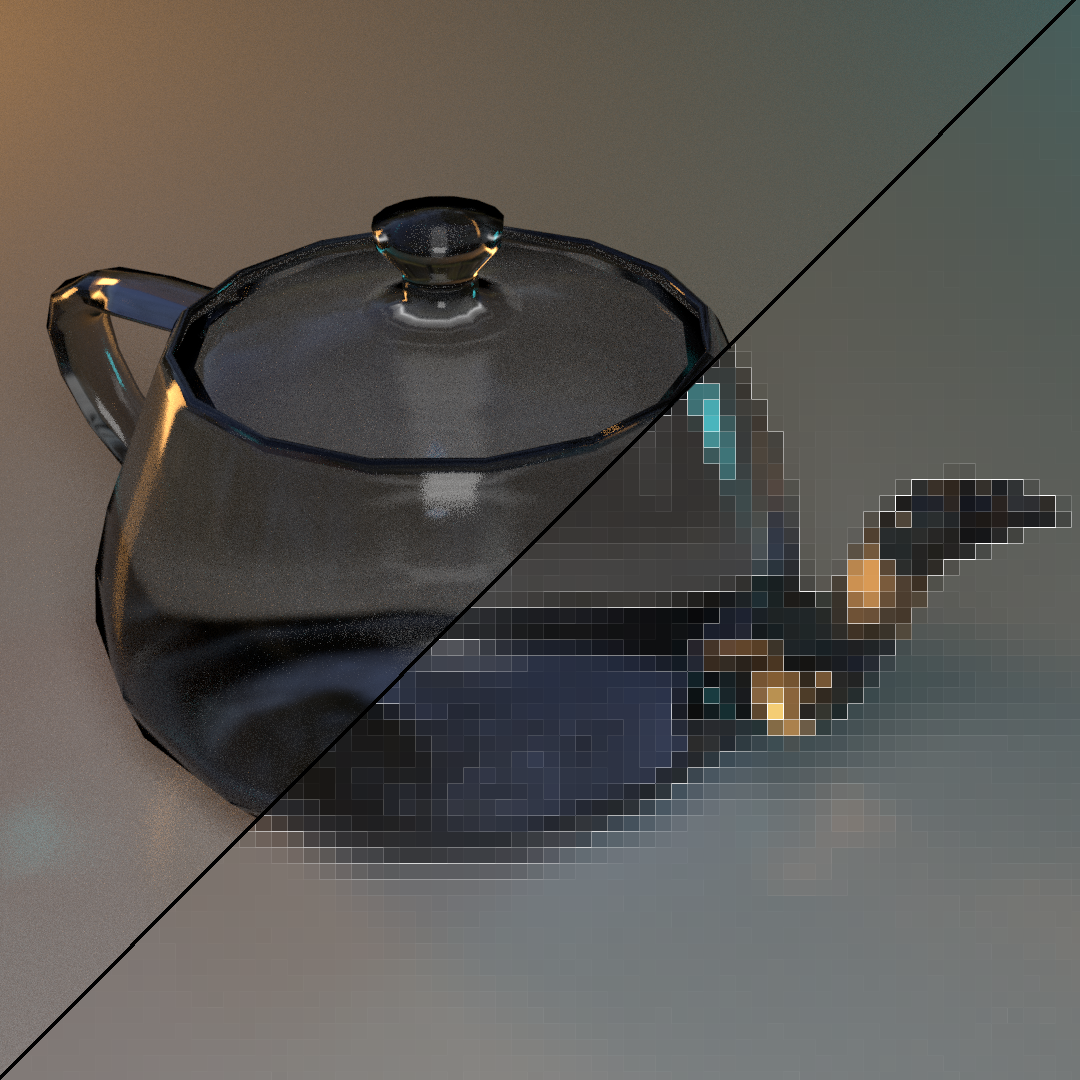
\includegraphics[width=4cm]{graphics/teapot_rt_pix}} \\
    
    \bigskip

    Computer graphics is the science of turning \textit{shapes} into \textit{pixels}.
\end{center}
\end{frame}

\begin{frame}{Uses}
    \noindent
    \begin{minipage}{.65\textwidth}
        Computer graphics is everywhere!
        \begin{itemize}
            \item Your terminal \\
            \item Web browsers \\
            \item Video games \\
            \item CAD software \\
            \item Movies, TV Shows \\
            \item Virtual reality \\
            \item Your bootloader \\
            \item QT, GTK+, wxWidgets \\
            \item Vim, Emacs, Notepad \\
            \item Embedded devices
        \end{itemize}
    \end{minipage}% This must go next to `\end{minipage}`
    \begin{minipage}{.35\textwidth}
        \pmidg{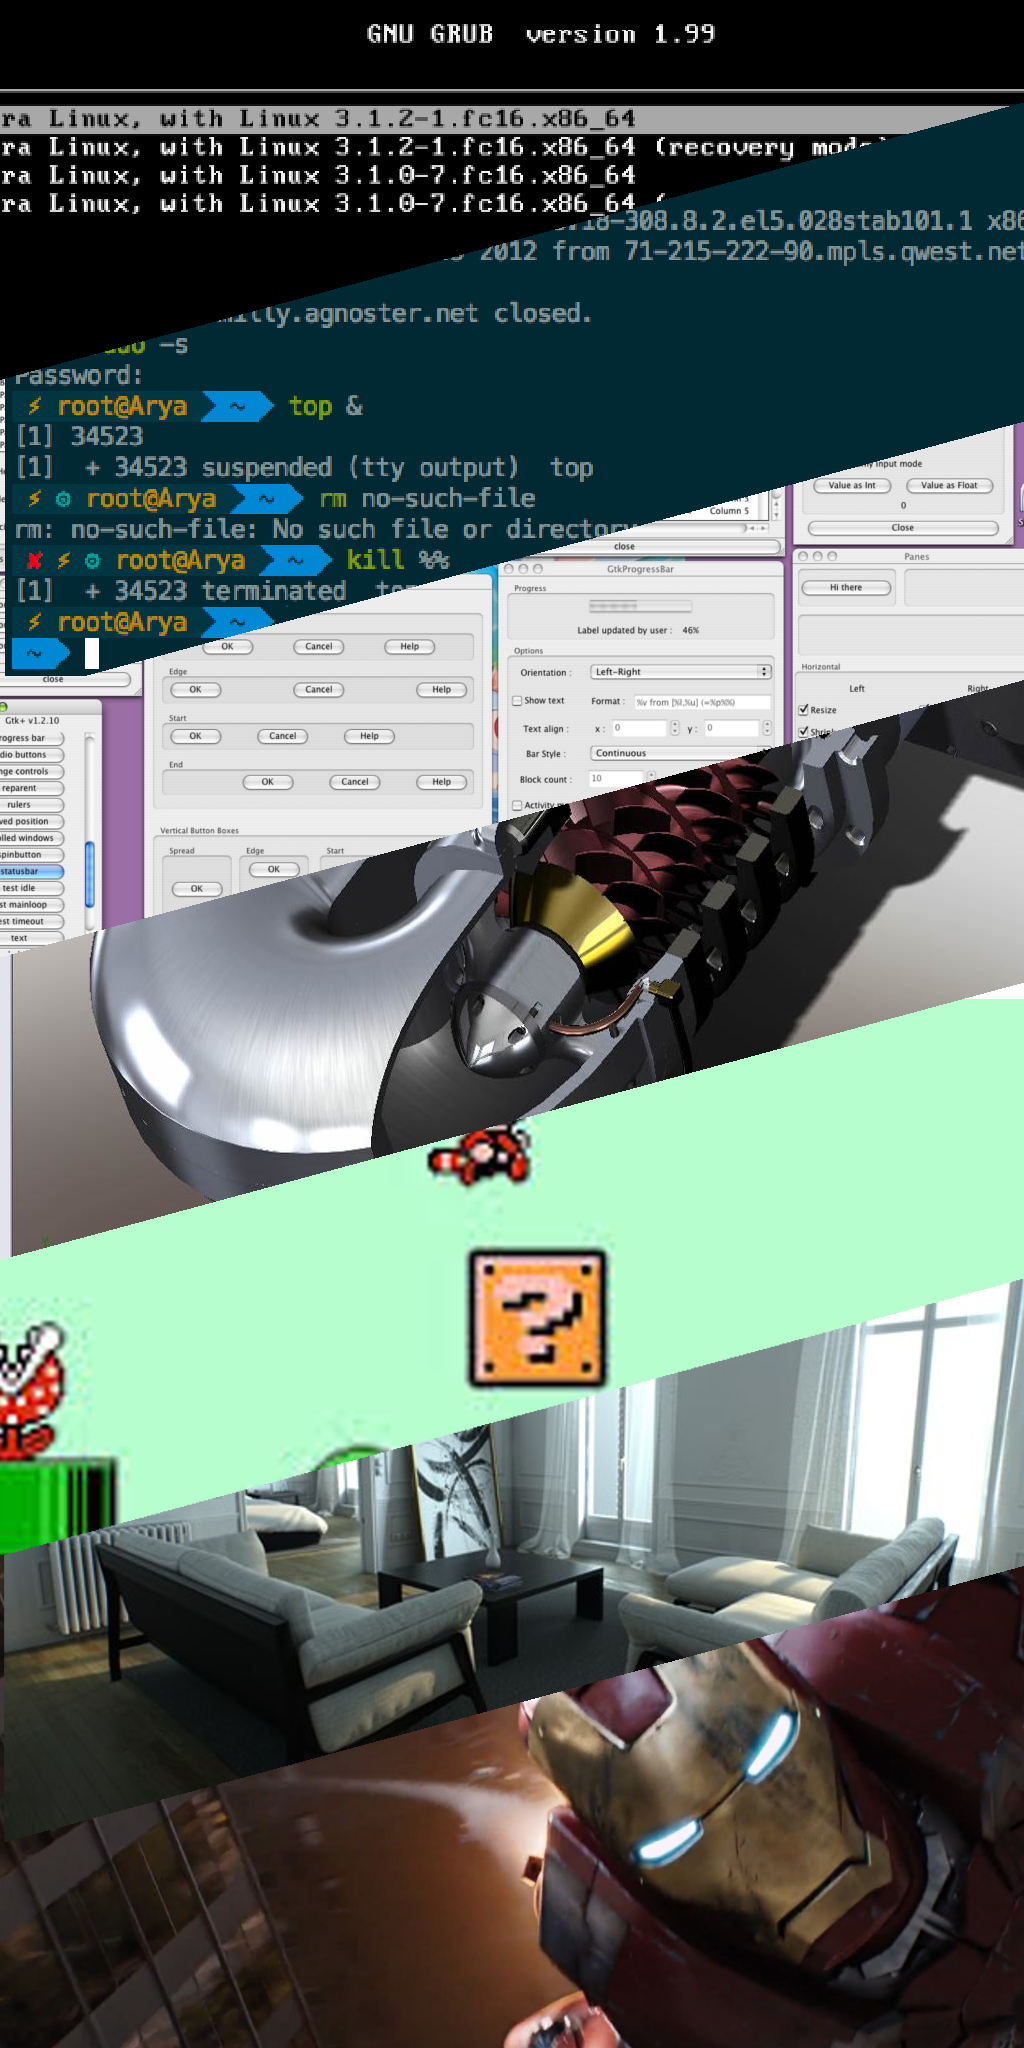
\includegraphics[width=\textwidth]{graphics/uses}}
    \end{minipage}
\end{frame}

\begin{frame}{Online and Offline}
\end{frame}

\begin{frame}{History}
\end{frame}

\end{document}
